\documentclass[twoside,11pt]{article}

% Any additional packages needed should be included after jmlr2e.
% Note that jmlr2e.sty includes epsfig, amssymb, natbib and graphicx,
% and defines many common macros, such as 'proof' and 'example'.
%
% It also sets the bibliographystyle to plainnat; for more information on
% natbib citation styles, see the natbib documentation, a copy of which
% is archived at http://www.jmlr.org/format/natbib.pdf

\usepackage{jmlr2e}
\usepackage{setspace}

% Graphics
\usepackage{graphicx}
\graphicspath{{images/}}

% algorithms
\usepackage{algorithmic}

% Definitions of handy macros can go here
\newcommand{\dataset}{{\cal D}}
\newcommand{\fracpartial}[2]{\frac{\partial #1}{\partial  #2}}

% Heading arguments are {volume}{year}{pages}{date submitted}{date published}{paper id}{author-full-names}
\jmlrheading{1}{2000}{1-48}{4/00}{10/00}{meila00a}{Christopher Jeschke}

% Short headings should be running head and authors last names

\ShortHeadings{Dissertation Critique}{Jeschke}
\firstpageno{1}

\begin{document}

\title{Dissertation Critique: Exploring Machine Learning Techniques Using Patient
      Interactions In Online Health Forums to Classify Drug Safety}

\author{\name Christopher Jeschke \email cjeschk2@jhu.edu \\
       \addr Engineering for Professionals\\
       Johns Hopkins University\\
       Elkridge, MD 20175, USA}

\editor{n/a}

\maketitle


% Entire paper should be single spaced
\singlespacing

% Abstract
\begin{abstract}%   <- trailing '%' for backward compatibility of .sty file
  Patient generated health data represents an area of active research interest
  for its potential applications in improving the public health. The study of
  Pharmacovigilance is one such area, focused on monitoring drugs once they have been released to market. Dr. Brant Chee's 2011 dissertation applying machine learning techniques to patient messages in online health forums explores how watch list drugs from the United States Food and Drug Administration's pharmacovigilance program can be detected via these forum messages, ultimately with the intent to alert consumers to drug safety concerns.
\end{abstract}

\begin{keywords}
  Drug Safety, Pharmacovigilance, NLP
\end{keywords}

\section{Summary of Research}
%Todo:  Fix Niave Bayes double dot
Dr. Brant Chee's 2011 dissertation \textit{Exploring Machine Learning Techniques Using
Patient Interactions in Online Health Forums to Classify Drug Safety} describes
Chee's research in applying natural language processing (NLP) techniques in conjunction with Na\"ive Bayes and Support Vector Machine classifiers to identify candidate \textit{watch list} drugs from online patient forums. Watch list drugs are identified by the United States Food and Drug Administration (FDA) as presenting a significant health or safety risk to drug consumers, prompting regulatory action to better inform the consumer or direct intervention by removing the drug from market. Chee's dissertation seeks to answer the specific questions:
\begin{itemize}
  \item Can Machine Learning classification methods using text features extracted from online health forums be used to identify FDA watch list drugs?
  \item Is the sentiment of the forum message useful in identifying these drugs?
  \item Similarly, are the drug effect entities useful in identifying watchlist drugs?
\end{itemize}

This research is accomplished through an empirical study using a corpus from the
Yahoo! public health forums. Chee develops NLP techniques to define and distill a feature space for classification using Na\"ive Bayes and
Support Vector Machine classifiers for detecting watchlist drugs. Drugs detected are evaluated against watchlist drugs found via the FDA Adverse Event Reporting System (FAERS) to determine the utility of the approach and its applicability in Pharmacovigilance. %GOOD

\subsection{Background: Pharmacovigilance, AERS and Social Media}
The dissertation begins with an extensive background discussion on adverse drug reactions and current surveillance techniques. Adverse drug reactions are defined by the FDA and World Health Organization (WHO) as "A response to a drug which is noxious and unintended and which occurs at doses normally used in man for prophylaxis, diagnosis, or therapy of disease or for modification of physiological function."\cite{FDA}. Chee continues by introducing Pharmacovigilance as "the study of drugs once released to market" \citep{Chee}, and the important regulatory agencies practicing it are mentioned - the World Health Organization (WHO) and United States Food and Drug Administration (FDA). The FDA Adverse Event Reporting system (AERS) is discussed and comparison with it is central to the work. AERS was constructed to house mandatory drug safety reports from drug manufacturers, distributors and health care facilities, as well as voluntary reports submitted by patients, physicians and other healthcare providers.
Chee identifies a major limitation in AERS and other \textit{spontaneous reporting systems} in that they are known to have high underreporting rates \citep{Fletcher}, due to the likelihood of a patient reporting an event only if they feel their healthcare provider has not paid attention to the adverse drug reaction observed \citep{Leamon}. Social media provides a venue for patients to share their health information in anonymous setting as patients are not always transparent nor truthful with their physicians. Online health forums create an environment where patients can find those having similar backgrounds, conditions and challenges, prompting rich social interactions where patient disclose their opinions and observations about their current drug regimen effectiveness and perceived adverse effects. Chee feels these forums represent an untapped means to crowdsource data for the pharmacovigilance task. %Reviewed

\subsection{Experimental Data}
The data selected for the dissertation's experimentation is a Yahoo! corpus containing 12.5 million messages from various Yahoo Health group forums. As the data is a raw export containing a combination of message metadata, raw text and HTML, it must first be studied to better understand its composition and what NLP techniques will be applied for feature extraction. %Reviewed

\subsubsection{Tokenization Study of Data}
Chee conducts an initial study of the Yahoo! corpus by selecting at random 500 messages, stripping them of html tags, numerical and punctuation only tokens (\$, \%, :), :(, etc), then tokenizing them on white spaces with trailing punctuation. The tokens are evaluated in several rounds of classifiction using lexicons constructed by Chee to aid in understanding message composition. Lexicons for English and foreign language were drawn from the OpenOffice project \citep{OpenOffice}, drug names from the Drugs@FDA website, medical and disease terminology from terms on MedicineNet and Wikiepedia, and a MedDRA lexicon from FDA AERS. A names lexicon was constructed using person names harvested from various sources. The classification process was iterative. If a token did not initially classify via a lexicon, it was manually classified into \textit{error types}. Average metrics were as follows:
\begin{center}
  \begin{tabular}{||c|c||}
    \hline
    \verb|Average # of Tokens per Messsage:| & 172.21\\
    \hline
    \verb|Average # of Drug Name Tokens:| & .29\\
    \hline
    \verb|Average # of Error Type Tokens:| & 7.09\\
    \hline
    \verb|Average # of Name Tokens:| & 5.34\\
    \hline
    \verb|Average # of Medical Tokens:| & .81\\
    \hline
  \end{tabular}
\end{center}
Of the error tokens, over 54\% of them were found to be foreign language tokens - primarily Indonesian and Spanish - motivating subsequent experimentation to classify messages as English before incorporating them into later studies. Spelling errors were also a concern, but the classification results show only a $.8\%$ error rate. %Reviewed.

\subsubsection{A Vocabulary for Experimentation}
Chee cites performance concerns training classifiers using all the words in the message as this would expand the feature space. Additionally, multiple words together in order can convey a different meaning than separate single words, such as "vitamin a" compared to "vitamin" and "a". These constraints motivate the use of word-grams - unigrams, bigrams and trigrams specifically - as a way to capture more accurate meaning. Specialized lexicons are developed to ensure the classifiers do not overfit to drug names and generalize to considering drug effects, sentiment and other terminology. The lexicons are:
\begin{itemize}
  \item drugs - a drug list from drugs.com
  \item medical - medical terminology extracted from MedicineNet
  \item sentiment - a sentiment lexicon from the combination of SentiWordNet and Linguistic Inquiry and Word Count (LIWC)
  \item medra - the MedDRA terms for drug adverse events/outcomes from FDA AERS
  \item disease - a disease list from Wikipedia
\end{itemize}
These five lexicons allow for twentynine different datasets of features to be constructed from the Yahoo! corpus messages for the watchlist drug classification experiments. %Reviewed

\subsection{Language Identification for Messages}
The tokenization study identified a significant number of foreign language messages in the corpus which Chee aims to eliminate to reduce the feature space. Messages containing non-romanized text are removed first using Unicode language detection. Messages in non-English languages in romanized text are harder to discern. Dictionaries for English and foreign languages are taken from the OpenOffice project and used in conjunction with the medical, drug, disease and name lexicons mentioned earlier in an algorithm to obtain token counts. Once the counts are obtained, the following linear inequality is evaluated per message:
\[
  4 * foreign + unknown + ignore > english + drugs + medical
\]
The weighting of the foreign words is selected to ensure messages contain less than 25\% foreign words to be considered English. Only the English messages are retained, reducing the corpus to 10,178,710 messages and the number of unique terms per message from 2.5 to 2. %Reviewed

\subsection{Experimentation and Results}
The goal of the dissertation is to develop a classification system for drugs based on how people are talking about them in online message forums. Processed forum messages are first organized by drug, divided into test and training sets, converted into feature vectors, and then run through Support Vector Machine and Na\"ive Bayes classification algorithms. Chee conducts a multitude of these experiments using two versions of the feature vector structure, multiple combinations of the lexicons described earlier, the optional use of Bi-Nomial Separation to choose word n-grams, and optional cost-weighting and normalization within the classifiers.

\subsubsection{Class Separability Confirmed via Kullback-Leibler Divergence}
Chee begins with an initial experiment to determine how separable messages about watchlist and non-watchlist drugs will be in order to validate the classification approach. Kullback-Leibler divergence (KL divergence) is used to measure the difference in word frequency distribution between messages in each category. A smoothing technique is applied to make sure each term is represented in each distribution to avoid infinite divergence when terms are missing from one class. KL-Divergence between watchlist and non-watchlist word frequencies is calculated, and divergence from Google and Reuters corpi to provide perspective. The terms overexpressed in the watchlist messages are also examined:
\begin{center}
  % KL Divergence Metrics
  \tabular{||c|c|c|c|c||}
    \hline
    Classification & Watchlist & Non-Watchlist & Google & Reuters \\
    \hline\hline
    Watchlist & n/a & .1684 & 1.4178 & 1.3279 \\
    \hline
    Non-Watchlist & .1778 & n/a & 1.1804 & 1.0815 \\
    \hline
  \end{tabular}
  \quad
  \begin{tabular}{||c|c||}
    \hline
    Term & Divergence \\
    \hline\hline
    i & .007875 \\
    \hline
    my & .003018 \\
    \hline
    me & .0002256 \\
    \hline
    you & .001712 \\
    \hline
    i'm & .000964 \\
    \hline
  \end{tabular}
\end{center}
Clearly watchlist & nonwatchlist diverge, and show a different degree of divergence from the Google and Reuters corpi, indicating some separability. The overexpressed terms are interesting, as they seem indicative of emotional writing - just the kind that might occur when discussing a drug with an adverse effect.

\subsubsection{Named Entity Recognition in Messages}
Another challenge presented by Chee is how to identify the drugs and adverse events in a message - a problem of Named Entity Recognition (NER). A Lucene index is built atop the processed Yahoo! corpus, against which query phrases built from the drug and reactions lexicons are issued to determine term prevalence. A lower case filter with stemming is used, requiring that drugs containing common words (e.g. "commit" for the drug Commit) are replaced with their generic chemical names in the lexicon. Plots are produced showing term distributions:

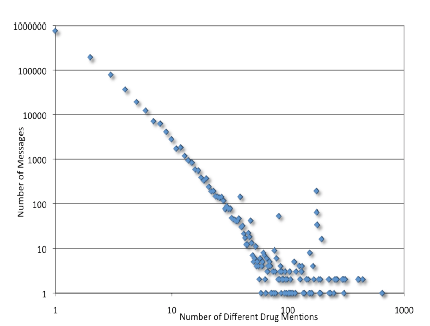
\includegraphics[width=7cm, height=5cm]{Figure-1-Zipfian.png}
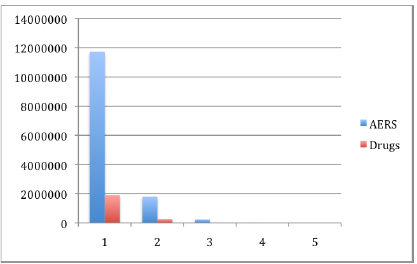
\includegraphics[width=7cm, height=5cm]{Figure-2-AERS_Drugs.png}

The first plot demonstrates a Zipfian distribution for drug name mentions in the messags, with more than 96\% of messages mentioning at most 5 drugs, prompting the elimination of messages having more than 5 unique drugs as these tend to be lists or SPAM. The second plot shows that adverse events are mentioned far more often than drug names. It is suggested that a preceeding post containing a drug name eliminates referencing it in subsequent posts that are replies, but this is an area for future research. If multiple drugs are mentioned in a single message it becomes difficult to discern which drug the message should apply to, so another study is done to evaluate the distance (number of characters) between the top 25 co-occuring drugs. A Zipfian distribution is observed for character separation, suggesting drugs are talked about within the same or across adjacent sentences, making separation difficult. Therefore, messages are attributed to all drugs mentioned. %Reviewed

\subsubsection{Sentiment Feature}
 Chee hypothesizes that the positive or negative valence in a message represents drug satisfaction, making it an interesting feature to incorporate into the classification experiments. A lexicon using positive emotion, negative emotion, anxiety, anger and sadness terms from LIWC is constructed, augmented with several emoticons (:), :(, ..) and acronyms (LOl, ROFL, ..). Two case studies are then executed using messages sampled from specific groups in the corpus, and the change in drug sentiment is analyzed over the drug's pre-recall, recall, and post-recall timesframes against a control sentiment derived from messages not containing the drug.

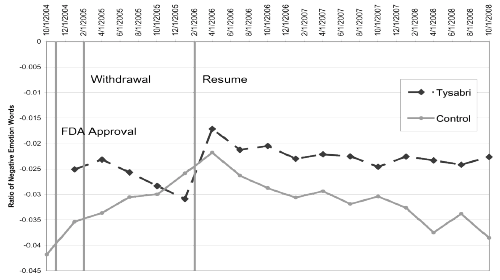
\includegraphics[width=7cm, height=5cm]{Figure-3-Tysabri.png}
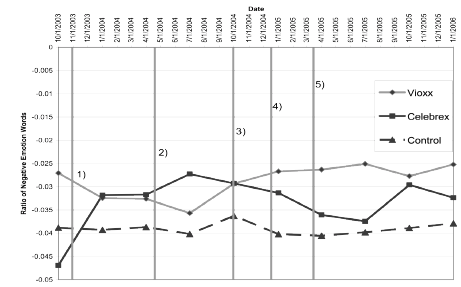
\includegraphics[width=7cm, height=5cm]{Figure-4-Vioxx.png}

The left-most plot shows the sentiment change for Tysabri pre-recall, recall and post-recall over the control. It shows a reasonably intuitive change in negative valence when Tysabri is introduced (more positive), withdrawn (negative), reintroduced (hopeful therefore positive), finally stabalizing. The right plot shows sentiment change for a pair of commonly used pain relievers - Vioxx and Celebrex - over the course of several public anouncements. First a withdrawal of Viox (sections 1 through 3), then Celebrex (4 and 5). ANOVA is applied, determining statistical significance against the control with p < .001.

\subsubsection{Feature Selection, Training and Test Data Size}
The introduction to the main body of classification experiments is preceeded by a brief discussion on the features vectors used, as well as how training, test and validation sets are constructed to support the use of 10-fold Cross Validation for classifier evaluation.
Two types of feature vector are decided upon and then leveraged in the  experiments. The first is generated over general vocabulary terms in the messages selected based on frequency cutoffs. The vector is augmented with counts from the specialized lexicons: medical, diseases, drugs, sentiment and reactions (MedRA). The second feature vector uses only the specialized lexicons to identify the word features.
The richness of the training data is of foremost concern, as there are only 435 drugs having 500 or more unique messages, and only 575 drugs having more than 250 messages, with 63 and 77 watchlist drugs mentioned in each respectively. Approximately 90\% of message instances reference non-watchlist drugs, creating a data scarcity problem when attempting to classify watchlist drugs. Chee decides upon a minimum cutoff of 250 messages per drug. An experiment is constructed to evaluate techniques to address the scarcity, including scaling features, selecting different ratios of negative to positive training examples, and experimenting with different split ratios in cross-validation - 90/10 and 80/20. These experiments are deamed inconclusive and not elaborated on further.

\subsubsection{Classifier and Lexicon Selection}
The next goal of the dissertation's experimentation is to discover the best performing combinations of classifier, lexicons and feature selection as a means to inform the construction of a \textit{meta classifier} to be used in watchlist drug prediction. The inconclusive nature of the data set sizing experiments prompts settling on the following methodology for classifier
training and evaluation:
%\begin{itemize}
%  \item Test and training sets are sampled with the same distribution as the original data. No use of 1:1, 2:1 or similar negative to positive ratios.
%  \item Data is divided into a 90/10 split, where 90\% of the samples are used to train and 10\% used to validate.
%  \item The splits themselves are sampled per the original distribution.
%\end{itemize}
The classifier evaluation experiments evaluate combinations of classifier type, the optional use of normalization and cost-weighting, and various combinations of lexicons. The experimental results and analysis make heavy use of acronyms to understand the combinations evaluated. For example, \textit{drugs\_dis\_sent\_react\_NSVMC} would equate to an experiment using a Normalized SVM with Cost Weighting (NSVMC) incorporating the drugs(drugs), disease(dis), sentiment(sent) and reaction(react) lexicons. A series of 240 experiments were run using the combinations above to ascertain the best combination of lexicons when evaluating accuracy, F1 score, and area under the ROC curve (AUC).The top 3 classifier configurations for accuracy are presented below with their upper and lower bounds:
\begin{center}
  \begin{tabular}{||c c c c||}
    \hline
    Configuration & Accuracy & Lower & Upper \\
    \hline\hline
    \verb|dis_react_NSVM| & 0.9032 & 0.7932 & 0.9578 \\
    \hline
    \verb|drugs_dis_sent_react_NSVM| & 0.9013 & 0.7908 & 0.9566 \\
    \hline
    \verb|drugs_sent_react_NSVM| & 0.9013 & 0.7908 & 0.9566 \\
    \hline
  \end{tabular}
\end{center}
The accuracy of a naive baseline classifier that labels all instances as negative would be 86.7\% per concentrations of non-watchlist and watchlist drugs in the training data. While several configurations exceed this, when considering the lower bound there is uncertainty that any classifier is more accurate than the naive baseline. F1 and area under the ROC curve (AUC) scores are evaluated next:
\begin{center}
  \begin{tabular}{||c c||}
    \hline
    Configuration & F1 Score\\
    \hline\hline
    \verb|drugs_dis_react_NSVM| & 0.4761 \\
    \hline
    \verb|drugs_dis_react_UNB| & 0.4725 \\
    \hline
    \verb|drugs_UNB| & 0.4698 \\
    \hline
  \end{tabular}
  \quad
  \begin{tabular}{||c c||}
    \hline Configuration & AUC \\
    \hline\hline
    \verb|drugs_UNB| & 0.7592 \\
    \hline
    \verb|drugs_dis_UNB| & 0.7564 \\
    \hline
    \verb|med_drugs_NNB| & 0.7545 \\
    \hline
  \end{tabular}
\end{center}
Neither the F1 nor AUC scores are particularly impressive, though the experimental results do show lower F1 scores with cost weighting. The F1 scores were decomposed into their precision and recall components, then scatter plotted. The general observation was most scores had a mass concentration of low recall and precision, with the occassional high recall or high precision outlier - though never both.
As the goal of this experiment was to identify the value of the lexicons, their prevelance in the top 10 best performing weighted and non-weighted classifiers for each metric is examined:
\begin{center}
  \begin{tabular}{||c c c||}
    \hline
    Lexicon & Non-Weighted Classifiers & Weighted Classifiers \\
    \hline\hline
    Drugs & 33 & 20 \\
    \hline
    Disease & 32 & 18 \\
    \hline
    Sentiment & 28 & 15 \\
    \hline
    Reactions & 27 & 10 \\
    \hline
    Medical & 7 & 5 \\
    \hline
  \end{tabular}
\end{center}
The ranking favors the drugs, disease and sentiment lexicons, which are then selected for use in the prediction problem. This does raise overfitting concerns as the classifier will learn on drug names and diseases associated with watchlist drugs. It is disappointing that reactions doesn't rank higher, but it may not capture how people speak about adverse events.

\subsubsection{Evaluating the BNS Lexicon}
Another area of experimental exploration is how the initial word n-gram features are selected to populate the feature vectors. Bi-Normal Separation (BNS) is an alternative technique explored by Chee for discovering the word n-grams. BNS identifies those n-grams that are differentially expressed between two classes, in this case the watchlist and non-watchlist messages. BNS lexicons are constructed using the test subset of data for the top 15,000, 10,000 and 5,000 word n-grams, then tested in combination with the drugs, disease and sentiment lexicons, as well as additional "numerical features" containg counts for mentions of diseases, drugs, medical terms, sentiment and AERS terminology. Unfortunately the best BNS classifier underperformed the previous tests with an accuracy of only .8762 and lower bound of .7602. There was no clear advantage to BNS features nor the additional numerical features. The F1 and AUC scores for this test showed no improvement either, though un-normalized Na\"ive Bayes did have a higher F1 and AUC than normalized Na\"ive Bayes as seen above.

\subsubsection{Predicting Watchlist Drugs}
The previous experiments were used to assemble a meta-classifier using the best classifiers based on accuracy, F1 and AUC scores. The following were selected:
\begin{itemize}
  \item Normalized SVM using disease, reaction (AERS) lexicons with a 90.33\% Accuracy
  \item Normalized SVM using drugs, disease and reaction lexicons with an F1 score of 0.4762
  \item Un-Normalized Na\"ive Bayes with an AUC score of 0.7592
\end{itemize}
Two meta-classification experiments are constructed to examine the False Positives produced as an indicator for a possible \textit{future} watchlist drugs if used in an applied setting. The first experiment uses the classifier configurations stated above, but the training data is modified to denote drugs \textit{withdrawn} from the market as non-watchlist. It is important to distinguish that a withdrawn drug would have at one point been a watchlist drug, as drugs are placed on the watchlist - even if briefly - before being removed from the market. By looking for these withdrawn drugs marked non-watchlist in the set of False Positives from the training results, we evaluate the ability to discern new watchlist drugs. This experiment was executed via training runs to build 100 classifiers of each configuration. A scoring methodology is applied using the following linear combination:
\[
  \frac{\#\ of\ False\ Positives}{\#\ of\ Occurrences} * (\#\ of\ False\ Positives) * (\#\ of\ Classifer\ Types)
\]
Each occurence equates to an instance of the withdrawn drug actually being classified in the training. The table below shows the top 5 scores by generic drug name, as well as those withdrawn drugs identified as false positives.
\begin{center}
  \begin{tabular}{||c c c c c||}
    \hline
    Drug & # Positives & # Occurrences & # Classifiers & Score \\
    \hline\hline
    \textit{clozapine} & 31 & 64 & 3 & 45.047 \\
    \hline
    \textit{fludarabine} & 29 & 61 & 3 & 41.361 \\
    \hline
    \textit{methylphenidtate}(Ritalin) & 25 & 50 & 3 & 37.500 \\
    \hline
    \textit{morphine} & 15 & 38 & 3 & 15.474 \\
    \hline
    \textit{meloxicam} & 15 & 50 & 3 & 13.500 \\
    \hline\hline
    \textit{thalidomide} & 10 & 36 & 1 & 2.778 \\
    \textit{temazepam} & 11 & 50 & 1 & 2.420 \\
    \textit{hydromorphone} & 9 & 42 & 1 & 1.929 \\
    \textit{trovafloxacin} & 9 & 46 & 1 & 1.761 \\
    \textit{rofecoxib} & 9 & 50 & 1 & 1.620 \\
    \textit{sibutramine} (Meridia) & 5 & 27 & 1 & 0.926 \\
    \textit{cerivastatin} (Baycol) & 1 & 33 & 1 & 0.030 \\
    \hline
  \end{tabular}
\end{center}
The generic Sibutramine (brand name: Meridia) is of particular interest to this study, as it is under review but not yet an official watchlist drug. FDA has issued safety communications as of November of 2009, and the European Union has removed it from the market.

The second experiment entails removing the withdrawn drugs entirely from training, classifying them after a classifier is built for each fold during cross-validation. This approach is presumed to identify the withdrawn drugs with greater confidence as they are not present in the training data:

\begin{center}
  \begin{tabular}{||c c c c c||}
    \hline
    Drug & # Positives & # Occurrences & # Classifiers & Score \\
    \hline\hline
    \textit{methlyphenidate} (Ritalin) & 30 & 34 & 3 & 79.412 \\
    \hline
    \textit{morphine} & 13 & 38 & 3 & 13.342 \\
    \hline
    \textit{questiapine} & 14 & 31 & 2 & 12.645 \\
    \hline
    \textit{indomethacin} & 19 & 37 & 1 & 9.757 \\
    \hline
    \textit{sibutramine} (Meridia) & 17 & 34 & 1 & 8.500\\
    \hline\hline
    \textit{trovafloxacin} & 33 & 100 & 1 & 10.89\\
    \hline
    \textit{hydromorphone} & 33 & 100 & 1 & 10.89\\
    \hline
    \textit{rofecoxib} & 32 & 100 & 1 & 10.24 \\
    \hline
    \textit{thalidomide} & 10 & 36 & 1 & 2.778\\
    \hline
    \textit{temazepam} & 8 & 28 & 1 & 2.286\\
    \hline
    \textit{cerivastatin} (Baycol) & 2 & 100 & 1 & 0.04\\
    \hline
  \end{tabular}
\end{center}
Interestingly sibutramine does score significantly higher in this experiment, as do several of the withdrawn drugs (hydromorphone, rofecoxib, trovafloxacin), though Baycol scores much lower. Additionally, physiciatric drugs (Ritalin) and opiates (morphine) show up near the top in both experiments, presumably because they are more dangerous and more often associated with adverse reactions.


\section{Discussion of Contributions}
The major contribution of the dissertation is a collection of techniques for leveraging public health forum data for pharmacovigilance. Techniques in natural language processing and classification are developed and applied to identify drugs widthdrawn from the market by the FDA by using only the textual features of the messages themselves. The end result was an ensemble classification technique capable of identifying current watchlist drugs - and therefore \textit{future} watchlist drugs. In the interest of discussion, we can distill this work into several specific contributions worth individual discussion.

\subsection{Exploration and Annotation of Health Forum Data}
Chee's initial exploration of the Yahoo! corpus is informative in its own right, as it exposes the challenges in annotating messages from the general public for use in a scientific study. Scientific documentation - such as medical literature - is usually grammatically correct and highly precise in its use of scientific terminology such as drug names, diseases, side effects. Chee must confront a number of problems, including:
\begin{itemize}
  \item Differentiating between the message content and other artifacts, such as HTML tags, garbage strings, web URLs, and people's names
  \item Colloquial language, abbreviations and slang expressing sentiment, side effects and other medical terminology
  \item Misspellings to critical message content such as medical terminology and drug Names
\end{itemize}

The majority of message tokens contributing to these problems were placed in a general category of \textit{error}, accounting for 4.1\% of each message's tokens on average. This prompts a more in depth exploration into the nature of the errors, discovering that foreign languages appeared to be the largest contributor. However, the methods here did not go much further than identifying that problem tokens were present and attempting to classify them. If the nature of the problem token was known enough to classify them manually, why not replace them with a proper (grammatically correct) token of equivalent meaning, thereby preserving the value of the message? Mondern word processors frequently correcty for mispellings, and slang terminology such as "sux" could easily be replaced by a real world equivalent. Furthermore, these token type statistics were generated against only a 500 message sample of the corpus. It seems this kind of automated analysis could have been extended to encompas all messages in the corpus in order to confirm or deny these patterns.

\subsection{Techniques for Differentiating Language}
Chee's in depth analysis of the composition of health forum data identifies a high prevalance of foreign language terms in the messages. This is concerning, as these terms can inflate the word n-gram feature vector size going into the classifiers, motivating work to better classify messages as English or not. Chee starts by using Unicode language detection to take advantage of the most common website text representation: UTF-8 \citep{UTF_8 article on Wikipedia}. Characters not falling in the latin script code point range are eliminated.
Next, simple dictionary based methods using lexicons drawn from OpenOffice are used to classify tokens in a message as English or not for use later in message scoring. Other techniques are mentioned, but avoided for the following reasons:
\begin{itemize}
  \item The common words approach by \citep{Ingle, 1976} is mentioned, but given little attention.
  \item N-gram based techniques by Dunning \citep{Dunning} require training data, which he does not have. Furthermore, they can skew to repetitious words and phrases in online forums (e.g. "In Reply to")
  \item Character n-grams can't different between similar languages: Slovenian, Czech, Polish.
\end{itemize}

Dunning \citep{Dunning} does give some attention to the common words technique, stating these techniques are suitable when enough text is present to be classified as the common words are often \textit{closed class} words, with examples such as: and, or, this, that. These words often serve a function, such as joining other words and phrases thereby providing structure to the text. Sufficient amounts of text allow this structure to be identified and leveraged in classification. Dunning uses counter examples that are 20-characters long and 3-4 tokens to highlight the limitation, but considering the average 172 token length of the Yahoo! corpus it might have been more informative had Chee explored this technique further.

We could also advocate that Dunning's n-gram language classification technique would have been worth applying to develop a binary english-non-english classifier. Dunning develops his classification technique by modeling languages as a Markov Decision Process, wherein the probability of a particular word or phrase is dependent upon those preceeding it and their probabilities assuming a specific language. Dunning successfully differentiates between english and spanish texts of small length: 10, 20, 50, 100 and 200 bytes, having used relatively small training texts between 1000 and 50000 bytes. It seems reasonable that small sampling of longer, english only messages could have been identified as a training set to leverage this technique.

Additionally, recall the inequality $(4 * foreign) + unknown + ignore > english + drugs + medical$ used in message classification. Little beyond the initial token counts by type indicating foreign language prevalance and the resulting ~18.7\% reduction in message count thanks to the technique is provided as evidence of effectiveness. Chee himself noted that tokens can be part of multiple languages, yet the algorithm for counting tokens always favored English, likely skewing the counts. The vocabulary of the english language has been highly influenced by french and germanic languages \citep{Wikipedia page for english}, accounting for more than 55\%. This approach seems vulnerable to misclassification.

Finally, one would expect meta-data in the Yahoo! corpus messages might help discern the locality of the writer. Consider properties such as the name of the forum a message is under being english or not, or an IP address associated with a user being geo-resolvable to a US location.

While language classification is cited as a contribution of the dissertaton, the utility and accuracy of this approach is questionable.


\subsection{Named Entity Recognition: Drugs and Drug Effects}
Chee again favors dictionary methods for identifying drugs and drug effects within messages. The drug effects lexicon is composed from the FDA Adverse Event Reporting System (AERS), which uses the Medical Dictionary for Regulatory Activities (MedDRA) when coding reactions in the reports \citep{FAERS}. MedDRA has an onotological structure characterized by a top-most level of "System Organ Classes" (SOCs), two intermediate levels of high-level terms (term groups and terms themselves) falling within a SOC, followed in the the lowest levels by a preferred term (PT) and its synonyms, lowest level terms (LLT). It is the LLT or PT that may be recorded in a AERS report. Preferred terms are typically clinically correct, with the LLT being a more relaxed, colloquial phrase:
\begin{itemize}
  \item Nausea,  Feeling queasy
  \item Influenza,  Flu
\end{itemize}

The number of AERS (MedDRA) term instances found across the lucene indexed corpus of ~10M messages was 13,794,445. The experimental results published by Chee (Figure 13 in the dissertation) do show at least 1 AERS hit per message, indicating this approach worked and may be viable for recognizing adverse reactions in online, english text.

The results for drug identification were less promising.  The drug lexicon was composed from the FDA and a drugs taxonomy on Drugs.com. Chee outright states limitations in this approach as it does not account for all therapeutic biologicals, foreign names of drugs, nor the names of drugs not approved for US use. The volume of drug mentions was considerably less than the total number of messages, at 2,228,588. Several challenges make it difficult to discern the presence of a drug in a message:
\begin{itemize}
  \item limitations of the lexicon
  \item some drugs having brand names that are common words (e.g. Commit, used for curbing smoking habits)
  \item slang or colloquial terms
\end{itemize}

Without a broader lexicon, it is difficult to claim this method is successful at identifying drugs in messages. Low volume of drug identification in messages is one of the chief limitations of the work, in that very few watchlist drugs (77) were found, restricting the volume of training data.

Finally, the dictionary based approach looks only for the presence of a token in a message. It does not leverage the value that Part-of-Speech (POS) tagging could provide by differentiating between nouns (drugs), verbs, adverbs and other word categories.


\subsection{Feature Generation using BNS, Speciality Lexicons}
The Bi-Normal Separation (BNS) lexicon experimentation was intended to determine if word features (n-grams) expressed differently between watchlist and non-watchlist messages could serve as useful features in differentiating between the two classes. A study by Forman \citep{Forman} showed strong preference to BNS for feature in text classification for its ability to deduce word features occuring with greater prevalence in one class vs. another. Unfortunately the BNS experiments actually showed worse results compared to the use of the specialized lexicons by themselves. There were some methodological issues in the testing worth discussing:
\begin{itemize}
  \item the BNS lexicons were constructed using the test subset of the data, representing only 10\% of the Messages
  \item each BNS lexicon (5k, 10k, 15k) was tested in conjunction with the other speciality lexicons
\end{itemize}

The former was intentional to avoid biasing the classifier to just the Yahoo! corpus, but at the same time may have contributed to the poor performance of the classification experiments relative to non-BNS tests due to the reduced sample size. The inclusion of the speciality lexicons appears to have been done because this test followed the initial testing on the speciality lexicons only. At no point do we get to see the BNS selected n-grams in isolation.

The sentiment lexicon was another disappointment. While isolated evaluation with certain drugs (Tysabri, Vioxx) showed some changes in sentiment relative to a drug's watchlist status, sentiment did aid in greatly distinguishing messages as pertaining to watchlist or non-watchlist drugs. Chee hypothesizes this is because drug sentiment could be positive for drugs treating difficult illness despite significant side effects.

The drug and disease lexicons provide the best classifier performance. This is concerning because it could cause a classifier to overfit to drug names, hindering its ability to predict new watchlist drugs. Overall, the disertation seems to have been unsuccessful in finding a clear set of word features to separate watchlist from non-watchlist drugs.



\subsection{Quality of Watchlist Predictions}
Initially one would not be satisified with the minimial difference in accuracy shown between a naive classifier classifying each drug as non-watchlist (86\%) versus the accuracy observed in some of the best trained SVMs (90\%). Furthermore, the F1 and AUC scores were that exciting either. However, consider how these scores are defined:
\[
  Accuracy = \frac{TP + TN}{TP + TN + FP + FN}
\]
\[
  F1 = 2 \cdot \frac{precision * recall}{precision + recall}, \ precision = \frac{TP}{TP+FP},\ recall = \frac{TP}{TP+FN}
\]
\[
  AUC = P(X_{1} > X_{0})
\]
TP, TN, FP, FN stand for true positive, true negative, false positive and false negative respectively. For AUC, $X_{0}$ and $X_{1}$ are the classifier scores of randomly chosen positive and negative instances, and therefore an AUC = 1 represents perfect classification. A naive classifier assuming all instances were negative (non-watchlist) would have AUC and F1 scores of 0 and contribute nothing towards the goal of discovering future watchlist drugs. Additionally, note that each performance metric places value on the distinction between a true positive and a false positive, yet false positives are the means by which the value of the approach is communicated.  While it is counterintuitive to say a false positive result is diserable, the detection of a future watchlist drug via this technique would be represented as a false positive. Drugs do not become watchlist drugs until labeled so by the FDA. It might have been interesting had Chee presented and experiment those classifiers having the highest \textit{recall} rates though as observed, these frequently had very low precision would likely have contributed significant numbers of false positives that are just noise - drugs not bound for the FDA watchlist.

Chee's technique was successful in identifying a number of drugs withdrawn from the market despite their having been labeled as non-watchlist:  Palladone,  Trovan, Vioxx, and Baycol. Futhermore, the discovery of \textit{Sibutramine} (Meridia) was compelling because the time frame of the data set used stopped one year before Meridia was placed on a watchlist, demonstrating the ability to detect future watchlist drugs. It is far better to accidentally label a drug as a false positive, watchlist candidate than mistakenly mark it as false negative, failing to call attention to it and allowing considerable, sometimes deadly health consequences to go unnoticed.

The technique in this dissertation is not perfect by any means, but the approach developed does hold value as an augmentation to existing pharmacovigilance programs and techniques. The FDA AERS program is highly dependent on required reports filed by drug manufacturers and voluntary reports form health care providers, patients and their stakeholders \citep{FDA Aers}, and can in no way characterize the true incidence rate of adverse events in the U.S. population. Public health forums represent an interesting data source given how people are more likely to disclose health issues in a comfortable, social setting with peers, and the low barrier of entry for contributing to these conversations.


\section{Techniques and Algorithms}
Summarized herein are the technical details regarding the techniques and algorithms Chee used in his study, particularly as they pertain to feature selection and classification.

\subsection{KL Divergence}
Kullback-Leibler (KL) divergence quantifies the difference between two probability distributions. Given two distributions P and Q, it is expressed as:
\[
  D_{KL}(P||Q) = \sum_{i}P(i)log\frac{P(i)}{Q(i)}
\]
Where $P$ and $Q$ are probability distributions for two classes, $i$ is a value within each class, and $P(i)$ and $Q(i)$ are the probability of $i$ in each distribution respectively. Care must be taken that if $i$ is not present in $Q$, infinite divergence would occur, and so a low, default probability for $Q(i)$ may be used.

\subsection{Bi-Normal Separation}
Bi-Normal Seperation (BNS) is introduced as a word feature selection technique for use text classification. An empiral study by \citep{Forman} showed considerable performance advantages when using BNS with SVMs for text classification, as opposed to other selection metrics such as Information Gain (IG), Document Frequency (DFreq) and Odds Ratio (Odds). Testing with BNS had higher F1, precision and recall despite dealing with significant class skew in the training data on the order of 1:31 - 1 positive to 31 negative class examples. BNS is defined as:
\[
  F^{-1}(tpr) - F^{-1}(fpr)
\]
where $F^{-1}$ is the inverse of the normal cummulative distribution function, $tpr$ and $fpr$ are true and false positive rates respectively. Special exception is given to $F^{-1}(0)$ by defaulting to 0.0005 to avoid undefined values. The occurence of a feature (word) in a document is modeled by a random normal variable exceeding a threshold, with the prevalence rate of the word corresponding to the area under the curve after that threshold. A word expressed differently in the postive and negative classes will have different prevalence and therefore different thresholds, thus this metric measures the distance between the two thresholds.


\subsection{Support Vector Machines}
Support Vector Machines (SVM) \citep{Cortes, Vapnik} are well established for their utility in classification problems. An SVM functions by discovering a hyperplane that maximizes the margin of seperation between two classes given their feature space. The boundary lines of this hyperplane are identified as the \textit{support vectors}, being the vectors representing the training samples producing the best class separation. The simplest SVM finds the optimal hyperplane (w,b) satisfying the inequality:
%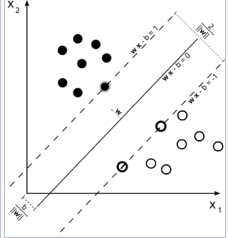
\includegraphics[width=7cm, height=5cm]{SVM.png}
\[
  y_{i}(w \cdot x_{i} + b) \gte 1,  i = 1, ...., l
\]
Where l = n, the number of training samples, and each training sample is a tuple $(x_{i}, y_{i})$, with $x_{i}$ the feature vector, $y_{i} = 1$ indicates membership of the positive class (watchlist) and $y_{i} = -1$ indicates membership of the negative class (non-watchlist). The optimal hyperplane is the tuple $(w, b)$ where $w$ is a vector and $b$ a scalar value. If $(w, b)$ are successfully found we have a \textit{hard margin} SVM classifier.

Rarely are classes so perfectly separable, so Chee opts to use a \textit{soft margin} SVM, allowing for a certain amount of classificaton error $\xi_{i} \geq 0$ on each training sample:
\[
  y_{i}(w \cdot x_{i} + b) \geq 1 - \xi_{i}
\]
with the goal being to minimize $C\sum_{i=1}^{l} \xi_{i}$, with $C$ a specified parameter. Furthermore, the issue of seperability can be addressed via the \textit{kernel trick} - a technique of injecting a kernel function $\Phi$ to project $x_{i}$ into a higher dimensional space:
\[
  y_{i}(w \cdot \Phi{x_{i}} + b) \geq 1 - \xi-{i}
\]

The \textit{Gaussian Radial Basis Function} (RBF) is selected for the kernel, defined as:
\[
  \exp(-\gamma||x_{i} - x_{j}||^{2}),\ \gamma > 0
\]

The parameters $C$ and $\gamma$ must be specified when training the SVM. This dissertation utilizes a \textit{grid search} to find their best combinations when training SVMs.


\subsection{Naive Bayes Classification}
Naive Bayes Classification has been popular in SPAM detection \citep{Sahami, 1998} and textual classification in general. The fundamental assumption is that the features (word n-grams) are independently distributed from one another within the classes of interest.

This classification technique seeks to answer the question "What is the probability that a given document D belongs to class C?", expressed as the \textit{conditional probability} $p(C|D)$ - the probability of the class $C$ given the document $D$.

\textit{Bayes Theorem} allows the manipulation of conditional probability to express $p(C|D)$ as:
\[
  p(C|D) = \frac{p(C)p(D|C)}{p(D)}
\]
where $p(D|C) = \prod_{i}p(w_{i}|C)$ with $w_{i}$ representing the $i-th$ word in a given document. Consider that we have two classes $C_{wl}$ and $C_{nwl}$ for watchlist and non-watchlist respectively. Using Bayes Theorem, we can construct the rules:
\[
  p(C_{nwl} | D) = \frac{p(C_{nwl})}{p(D)}\prod_{i}p(w_{i} | C_{nwl})
\]
\[
  p(C_{wl} | D) = \frac{p(C_{wl})}{p(D)}\prod_{i}p(w_{i}|C_{wl})
\]
Binary classification in Naive Bayes makes use of a \textit{decision rule}. The \textit{maximum a posteriori} (MAP) rule was selected, which chooses the most probable hypothesis. We are then given a classifer defined as:
\[
  \hat{y} = argmax_{k \element {wl, nwl}} p(C_{k}) \prod_{i=1}^{n}p(x_{i}|C_{k})
\]

$\hat{y}$ is assigned the class label based on the $k$ chosen per the maximumization defined above.

\section{Literature Review}

\subsubsection{Health & Safety Literature}
Adverse reactions have long held the attention of health regulatory bodies such as the World Health Organization (WHO) and the United States Food and Drug Administration (FDA).  In 1967, the WHO initiated a research project to collect case reports from 10 countries to evaluate an international system for monitoring adverse drug effects \citep(WHO,1971), prompting the WHO Drug Monitoring Centre - now the Uppsala Monitoring Centre (UMC) - to establish an international Pharmacovigilance program. The FDA's Adverse Event Reporting System - AERS, now known as FAERS - has records of adverse event and drug combinations dating back as far as 1969, as part of the FDA's Pharmacovigilance efforts.

\subsubsection{Text processing}
Rude, Gortner and Pennebaker conducted a study of easy writing by currently depressed, formerly depressed and never depressed college students, with the hypothesis that terms indicating self-preoccupation such as "I" will be more prevalent in depressed individuals, as well as emotional terms with negative valence \citep(Rude, 2004). Their study did confirm the hypothesis, in that "I" specifically was used more frequently by currently-depressed students, though other pronouns referencing the self (me, myself, my) were not. The study did leverage the Linguistic Inquiry and Word Count (LWIC) textual analysis program used by Chee in constructing a sentiment lexicon.

Pang and Lee \citep(Pang, 2008) discuss the tools and implications of treating online opinions as a first class object - something we actively mine for and take value in. They conduct an extensive survey of approaches for opinion-oriented search geared towards freeform text in blogs and forums, where opinion and sentiment must be deduced directly from message content, without the assistance of meta-data such as rankings (e.g.  1 to 5 \textit{stars}). Drawing from the rankings relationship  Pang and Lee are able to characterize sentiment as a regression problem as these rankings tend to be oridinal. Extraction of textual features is discussed, comparing the value of term \textit{frequency} verus \textit{presence}, the former usually being term-frequency inverse document frequency (tf-idf) and the later a binary indicator that a word is present or not. Previous studies by Pang indicate the later shows better performance in sentiment classification, differentiating sentiment modeling from topic modeling, likely influencing Chee's approach to sentiment feature modeling. Pang and Lee's treatment of the topic is extensive, covering domain considerations, the unsupervised construction of sentiment lexicons and single/multi-document evaluation.

Named entity recognition (NER) is an area of particular relevance to this work, determining the presence of drug names, diseases, relationships and related terminology in text. Extracting this kind of information from biomedical text
is addressed by \citep{Rindsfleich et. all, 2009} through the development of EDGAR, a natural language processing system for discovering drug & gene relationships pertaining to cancer as documented in biomedical literature. EDGAR benefits heavily from using the Unified Medical Language System (UMLS) and MetaMap \citep{Metamap} - an already existing tool for identifying medical language in text. EDGAR leverages contextual elements and consistency in phrase structure to identify gene, cell and drug names, then construct relationship predicates between them (e.g. is\_resistant(gene, cell, drug)). However, this approach heavily leverages the grammatical consistency of these texts, making it less applicable for recognizing named medical entities in web data.

General entity recognition in web data is examined in \citep{Etzioni, 2005}, where the KnowItAll system is developed and discussed - an unsupervised, domain-independent system for information extraction from the Web. The system uses generalized extraction patterns to generate candidate facts - such as city names - which are then tested for truth using assistance from search engines queries to compute a pointwise mutual information statistic for the fact. Chee emulates some of these techniques through phrase queries to validate drug names found in the Yahoo! corpus.

\subsubsection{Technical Literature}
Forman's paper on feature selection metrics for text classification \citep{Forman, 2003} introduces the BNS techinque, comparing it to several other metrics:  Chi-Squared, Information Gain, Odds Ratio,  Log Probability Ratio, and Document Frequency. Forman's experimental method uses a data set of computer science paper abstracts categorized into classes intermingled with another text classification data set, producing a variety of test data sets having a skew ranging from 1:1 (1 positive class and 1 negative) to 1:100+ (more than 100 negative instances). Classification experiments using SVMs are run with features selected via the identified metrics. BNS shows a consistently superior F1 measure and accuracy in the tests, with exception given to IG when the number of features selected is restricted to between 20 and 50 and the class skew is low. Incidentally, Forman's analysis uses SVM only, citing the works of \citep(Yan & Liu, 1999), \citep(Joachims, 1998) and \citep(Dumais, et. al) as confirming that SVM is an "outstanding" method for text classification. \par SVMs are introduced by \citep{Vapnik}, introducing the fundamental concepts, and hard and soft margin classifiers. Joachim's paper on text categorization with SVMs \citep{Joachim} explains why SVMs are expected to work well for text categorization, highlighting their ability to handle a large feature space of several thousand relevant words where training sample vectors may be sparse. Joachim comparse SVM text classification using polynomial and RBF kernels against Na\"ive Bayes, k-NN, C4.5 and the Rocchio algorithm, showing consistently higher precision/recall break even points for the SVMs across two popular test corpus.\par Na\"ive Bayes classification is explored in the context of SPAM classification by \citep{Sahami, ??}, who evaluates Naive Bayes classifiers trained on combinations of message word features, message word features plus specific phrases, and word features with phrases and domain specific features (non-word) features thought to indicate spam. Classification results in the binary SPAM/no-SPAM setting showing 100\% precision when using the final combination tested on a corpus of 1789 labeled messages. Like other studies, Sahami employs feature selection techniques to manage the feature space, ignoring words that appear less than three times and selecting only the top 500 remaining words based on their mutual information scores relavent to the class labels.


\section{Application Areas}
Chee's techniques seem reasonably applicable as an augmentation to current Pharmacovigilance programs that currently use structured reporting systems in the context of regulatory reporting requirements. The opportunity to leverage public health forum data in safety signal detection could help in the earlier identification of watch-list candidate drugs for these programs to pay special attention to when monitoring established safety systems. A system of monitoring public forums in this fashion could leverage what is a far greater volume of data, and the tendency for people to disclose medical issues and sentiments more readily within peer groups. Public health forum data is not necessarily the only data set where this technique could be applied either. The techniques developed within this dissertation could be applicable to clinical notes in electronic health records, health surveys or similar unstructured data sources, and are potentially extensible to any medical product where adverse reactions could be associated: devices, biologicals (a separate classification of drug), procedures, or named treatment regimens.

Chee's exploration of the Yahoo! corpus message content is illuminating, identifying the difficulties with language recognition, colloquial phrases, and other message artifacts germane to only messaging. The lexicon techniques developed were simple and functional, but would need further development to generalize well. For example, recognizing slang is a compelling problem in its own right and therefore developing slang lexicons for various languages or domains could provide a valuable toolset for normalizing online messages to more grammatically correct text, against which already existing trained, supervised NLP machine learning techniques could be applied, thereby improving named entity recognition capabilities and perhaps the robustness of the overall technique.

Feature selection within the study is another application area to address. It was suprising sentiment did not have a stronger influence in the classification experiments, but the use of the disease and drug lexicons might have overfit trained classifiers to drug names and surpressed any significant contribution from sentiment. Revisiting sentiment (negative valence) as an initial feature to which additional features might be added/removed would be an interesting extension of the study. The case studies mapping sentiment change in known watchlist drugs were insightful and might point to another way of signaling a future watchlist drug. The failure of BNS word n-gram selection to provide any improvements in performance measures is disappointing given \citep{Forman} but might have been due to the experimental methods - a low number of messages sampled proportional to the overall training set, suggesting that revisiting this approach might help.

Finally, it is worth discussing that this technique is not limited only to problems in the health and medical domains. Consumer product safety in general could benefit from monitoring public forums in this fashion in order to identify products posing significant safety hazards. Thousands of consumer products for child safety - such as car seats and life jackets - are available for purchase by the general public. Regulatory agencies such as the National Highway Traffic Safety Administration (NHTSA) must evaluate products and post recall notifications, but despite best efforts unsafe products will still make it to market. Constructing similar monitoring systems for these agencies using public forums could help identify products in the market with previously unrecognized defects.

\newpage
\bibliography



\subsection{Citations}
https://www.fda.gov/Drugs/GuidanceComplianceRegulatoryInformation/Surveillance/AdverseDrugEffects/


Cortes, C. and Vapnik, V. (1995) Support-vector network. Machine Learning, 20, 273-297.




Ingle, Norman. (1976). A language identification table.
The Incorporated Linguist, 15(4):98:101.

Dunning, T. (1994). Statistical identification of language. Technical report, Computing
Research Lab - New Mexico State University.


Dunning, T. (1994). Statistical Identification of Language. Computing Research Laboratory,
New Mexico State University.

HTML language specification: https://www.w3.org/TR/html4/

MedDRA heirarchy:  https://www.meddra.org/how-to-use/basics/hierarchy

FAERS: https://www.fda.gov/drugs/guidancecomplianceregulatoryinformation/surveillance/adversedrugeffects/ucm2007060.htm

BNS:
G. Forman. An extensive empirical study of feature selection
metrics for text classification. J. Mach. Learn. Res., 3:1289–
1305, 2003


Rindfleich, T.C., Tanabe, L., and Weinstein, J.N. (2002). EDGAR: Extraction of drugs, genes and relations from the biomedical literature.  In Proc. Pacific Symposium on Biocomputing.


WHO, 1972
World Health Organization (1972). International drug monitoring: The role of national centres. Report of a WHO meeting, World Health  Organ. Tech. Rep. Ser. 498, 1-25.

Rude, 2004
Rude, S.S., Gortner, E.-M. and Pennebaker, J.W. (2004). Language use of depressed and depression-vulnerable college students. Cognition and Function, 18(8), 1121-1133.

Pang, 2008
Pang, B. and Lee, L. (2008). Opinion Mining and sentiment analysis.  Foundations and Trends in Information Retrieval, (1-2),1-135.

Etzioni, O., Cafarella, M., Downey, D., Popescu, A. -M., Shaked, T., Soderland, S., Weld, D.S. and Yates, A. (2005). Unsupervised named-entity extraction from the web: An experimental study.  Artificial Intelligence 165: 91-134, Essex: Elsevier Science Publishers.

%joachims
@InProceedings{10.1007/BFb0026683,
author="Joachims, Thorsten",
editor="N{\'e}dellec, Claire
and Rouveirol, C{\'e}line",
title="Text categorization with Support Vector Machines: Learning with many relevant features",
booktitle="Machine Learning: ECML-98",
year="1998",
publisher="Springer Berlin Heidelberg",
address="Berlin, Heidelberg",
pages="137--142",
abstract="This paper explores the use of Support Vector Machines (SVMs) for learning text classifiers from examples. It analyzes the particular properties of learning with text data and identifies why SVMs are appropriate for this task. Empirical results support the theoretical findings. SVMs achieve substantial improvements over the currently best performing methods and behave robustly over a variety of different learning tasks. Furthermore they are fully automatic, eliminating the need for manual parameter tuning.",
isbn="978-3-540-69781-7"
}


%Sahami
Sahami, M., Dumais, S., Heckerman, D., and Horvitz, E. (1998). A Bayesian approach to filtering junk e-mail.   AAAI'98 Workshop on Learning for Text categorization





Metamap:
https://metamap.nlm.nih.gov/

\vskip 0.2in
\bibliography{sample}

\end{document}
